%%%%%%%%%%%%%%%%%%%%%%%%%%%%%%%%%%%%%%%%%%%%%%%%%%%%%%%%%%%%%%%%%%%%%%%%%
% Antes de correr el código:
% 1. Ingresar al Menu
% 2. Cambiar la opción "Compiler" a XeLaTeX
% 3. Cambiar la opción "TeX live version" a 2020 (opacidad de la imagen)
%%%%%%%%%%%%%%%%%%%%%%%%%%%%%%%%%%%%%%%%%%%%%%%%%%%%%%%%%%%%%%%%%%%%%%%%%
\documentclass[10pt]{article}
\usepackage[T1]{fontenc}
\usepackage[utf8]{inputenc}
\usepackage[english]{babel}
\usepackage{listings}
\lstset{language=R}
\usepackage[a4paper]{geometry}
\usepackage[dvipsnames]{xcolor}
\usepackage[framemethod=TikZ]{mdframed}
\usepackage{graphicx,tikz}
\usepackage{array}
\usepackage{float}

\geometry{top=2.54cm, bottom=2.54cm, left=2.54cm, right=2.54cm}

\usepackage{url}
\usepackage{lipsum} 
\usepackage{wrapfig}
\usepackage{subcaption}
\usepackage{multicol}

%==========================================
%======     FUENTE PARA CÓDIGOS      ======
%==========================================
\definecolor{codegreen}{rgb}{0,0.6,0}
\definecolor{codegray}{rgb}{0.1,0.1,0.1}
\definecolor{backcolour}{rgb}{0.98,0.98,0.98}

\lstdefinestyle{mystyle}{
  backgroundcolor=\color{backcolour},   
  commentstyle=\color{codegreen},
  keywordstyle=\color{blue},
  numberstyle=\tiny\color{codegray},
  stringstyle=\color{codegreen},
  basicstyle=\ttfamily\footnotesize,
  breakatwhitespace=false,         
  breaklines=true,                 
  captionpos=b,                    
  keepspaces=true,                 
  numbers=left,                    
  numbersep=5pt,                  
  showspaces=false,                
  showstringspaces=false,
  showtabs=false,                  
  tabsize=2
}

%==========================================
%==========     ESTILO TITLE     ==========
%==========================================
\newcommand{\City}[1]{\def\City{#1}}

\makeatletter         
\renewcommand\maketitle{
\begin{flushleft}
{\textcolor{black}{\huge \bfseries \@title }}\\[1ex]
\rule{\textwidth}{0.6pt}\\
\end{flushleft}
\vspace{-0.5cm}

\begin{flushleft}
\textcolor{black}{{\large  \@author} }\\[2ex]
\end{flushleft} } % Note the extra }
\makeatother

%==========================================
%==========    ESTILO CAPTION    ==========
%==========================================
\usepackage{caption}
\captionsetup[table]{name=Tabla ,textfont={it}, labelfont={bf},
                     justification=centering,
                     width =\dimexpr \textwidth-0.5cm\relax}
\captionsetup[figure]{textfont={it}, labelfont={bf},
                      justification=centering, skip=2pt,
                      belowskip=-5pt}
                      
%==========================================
%==========     ESTILO ITEM      ==========
%==========================================
\renewcommand{\labelitemi}{$\bullet$} 
\renewcommand{\labelitemii}{$\circ$} 
\renewcommand{\labelitemiii}{$\cdot$} 

%==========================================
%===   	LINKS (Agregar Hyperlinks)     ====
%==========================================
\usepackage[style=apa,
            urldate=long]{biblatex} 
\addbibresource{Bib.bib}

\DeclareSourcemap{
  \maps[datatype=bibtex]{
    \map{
      \step[fieldsource=note, final]
      \step[fieldset=addendum, origfieldval, final]
      \step[fieldset=note, null]}
      }
}

\DefineBibliographyStrings{english}{urlseen = {Accessed }    
}

\usepackage[colorlinks=true,linkcolor=RoyalBlue,
            citecolor=RoyalBlue,urlcolor=RoyalBlue]{hyperref}

%==============================================================
%==============================================================
\title{ }

%%%%%%%%%%%%%%%%%%%%%%%%%%%%%%%%%%%%%%%%%%%%%%%%%%%%%%%%%%%%%%%
%%%%%%%%%%%%                 INICIO                %%%%%%%%%%%% 
%%%%%%%%%%%%%%%%%%%%%%%%%%%%%%%%%%%%%%%%%%%%%%%%%%%%%%%%%%%%%%%
\begin{document}

\begingroup
\let\clearpage\relax % prevent extra page breaks
\thispagestyle{empty}
\begin{center}
{\huge \bfseries Universidad de los Andes}

\vspace{25pt}
{\LARGE \bfseries Departamento de Ingeniería de Sistemas}

\vspace{15pt}

\includegraphics[width=100pt]{images/logo.png} 

\vspace{35pt}
{\LARGE \bfseries Laboratorio: Introducción a Redes de Datos}
\vspace{55pt}

{\Large \bfseries ISIS3204 - Infraestructura de Comunicaciones}

\vspace{15pt}
{\Large \bfseries Profesor - Yuri Andrea Pinto Rojas}

\vspace{100pt}
{\Large \bfseries Grupo 3: }

\end{center}

\begin{flushleft}
  \setlength{\parskip}{0pt}
  \setlength{\itemsep}{0pt}
  \hspace*{4cm}\large\bfseries Juan Esteban Quiroga - 202013216

  \hspace*{4cm}\large\bfseries Juan Manuel Rodriguez - 202013372

  \hspace*{4cm}\large\bfseries Andres Felipe Ortiz - 201727662
\end{flushleft}

\begin{center}
\vspace{60pt}

\Large\bfseries 2025-10
\end{center}

\mbox{}
\endgroup

\clearpage

\tableofcontents
\clearpage

%==============================================================
%=====================   4.1   ================================
%==============================================================

\section{4.1 Configuración del Direccionamiento de la red (servicio de DHCP e IPs estáticas)}

En esta primera parte del laboratorio se buscó garantizar que todos los dispositivos de la red tuvieran una dirección IP válida y adecuada para comunicarse. Para ello se combinaron configuraciones de tipo \textbf{estática} (en los servidores) y de tipo \textbf{dinámica} (para los clientes).

\subsection{Configuración de los servidores con IP estática}

Los servidores de la red requieren direcciones fijas porque ofrecen servicios (DNS, FTP, correo, web, DHCP) que deben estar siempre disponibles en la misma dirección. En cada uno se ingresó manualmente la configuración en la opción \textit{Desktop → IP Configuration}:

\begin{itemize}
    \item Server1 – DNS: IP: 192.168.1.2, Mascara: 255.255.255.0, Gateway: 192.168.1.1
    \item Server2 – FTP: IP: 192.168.1.33, Mascara: 255.255.255.0, Gateway: 192.168.1.1
    \item Server3 – Mail: IP: 192.168.1.34, Mascara: 255.255.255.0, Gateway: 192.168.1.1
    \item Server4 – HTTP: IP: 192.168.1.35, Mascara: 255.255.255.0, Gateway: 192.168.1.1
    \item Server5 – DHCP: IP: 192.168.0.254, Mascara: 255.255.255.0, Gateway: 192.168.0.1
\end{itemize}

\begin{figure}[H]
    \centering
    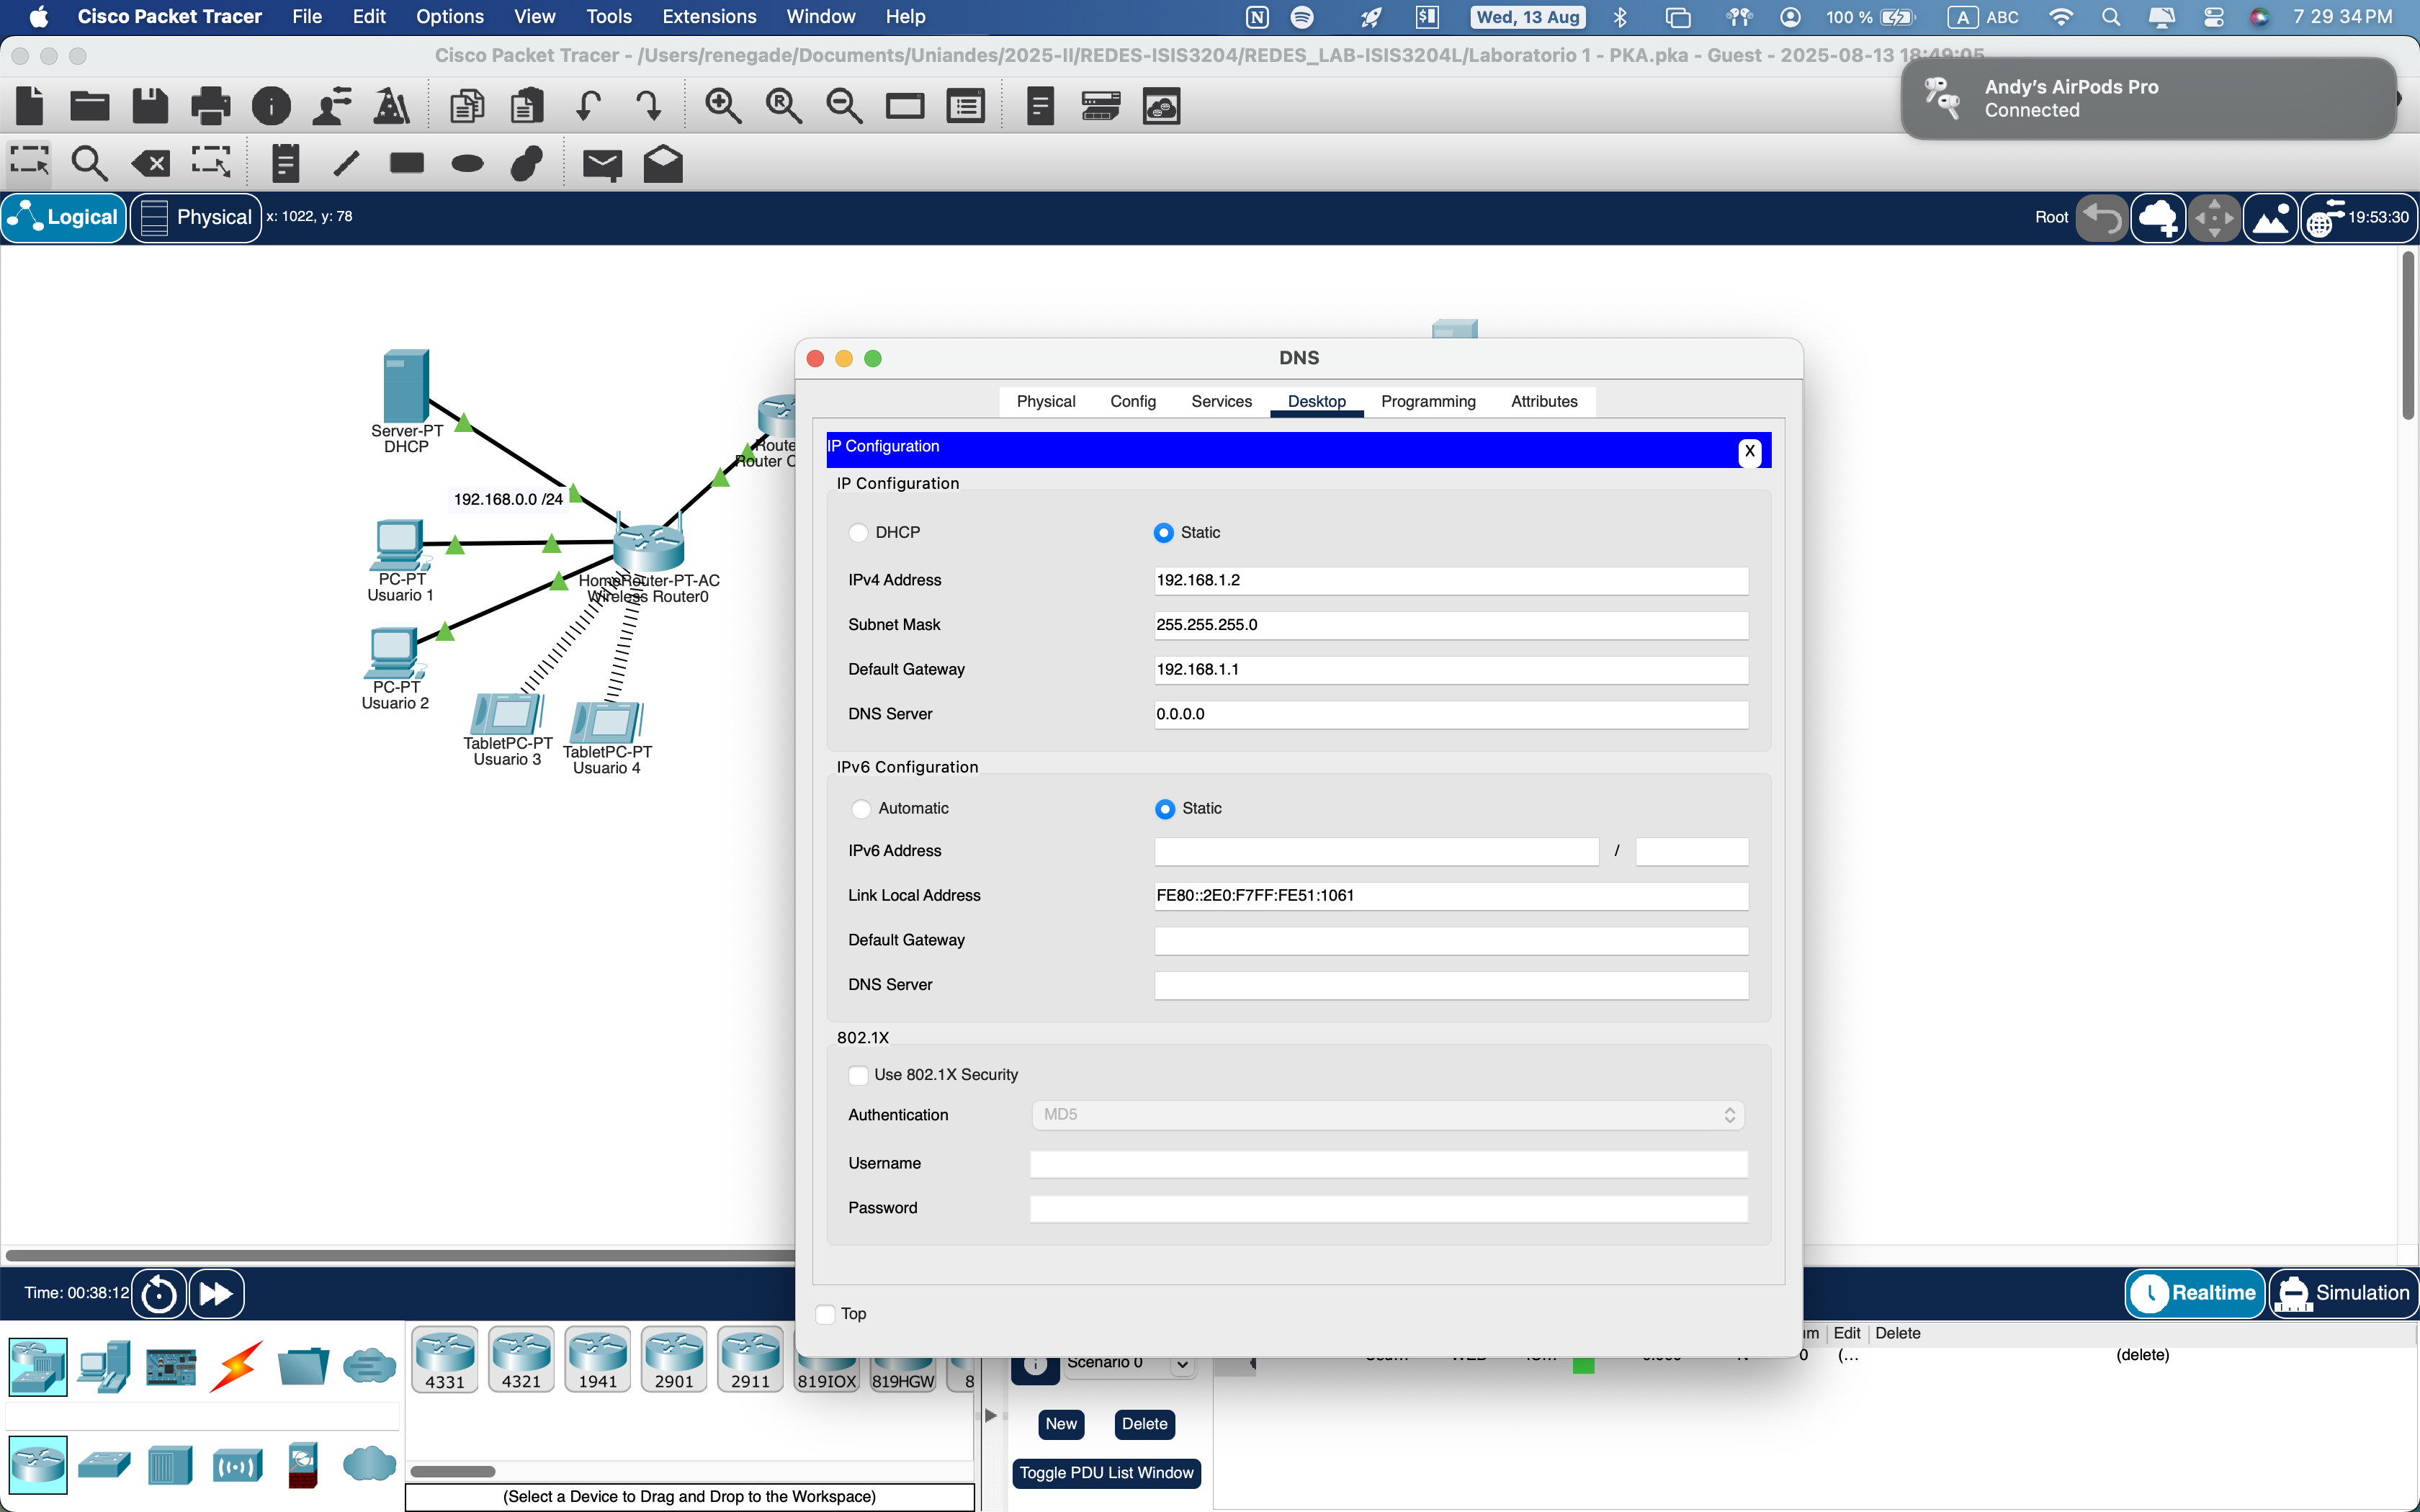
\includegraphics[width=0.65\textwidth]{lab-01-screenshots/41-1-DNS-ip-config.png}
    \caption{Ejemplo de configuración IP estática en el servidor DNS.}
\end{figure}

\subsection{Configuración del Servidor DHCP}

Para los clientes se habilitó un servidor DHCP en el Server5. De esta manera, los equipos de usuario obtienen su configuración automáticamente, lo cual simplifica la administración de la red.

El pool configurado contenía los siguientes parámetros:

\begin{itemize}
    \item \textbf{Default Gateway:} 192.168.0.1
    \item \textbf{DNS Server:} 192.168.1.2
    \item \textbf{Rango de direcciones:} 192.168.0.100 -- 192.168.0.255
    \item \textbf{Máscara de subred:} 255.255.255.0
    \item \textbf{Máximo número de usuarios:} 150
\end{itemize}

\begin{figure}[H]
    \centering
    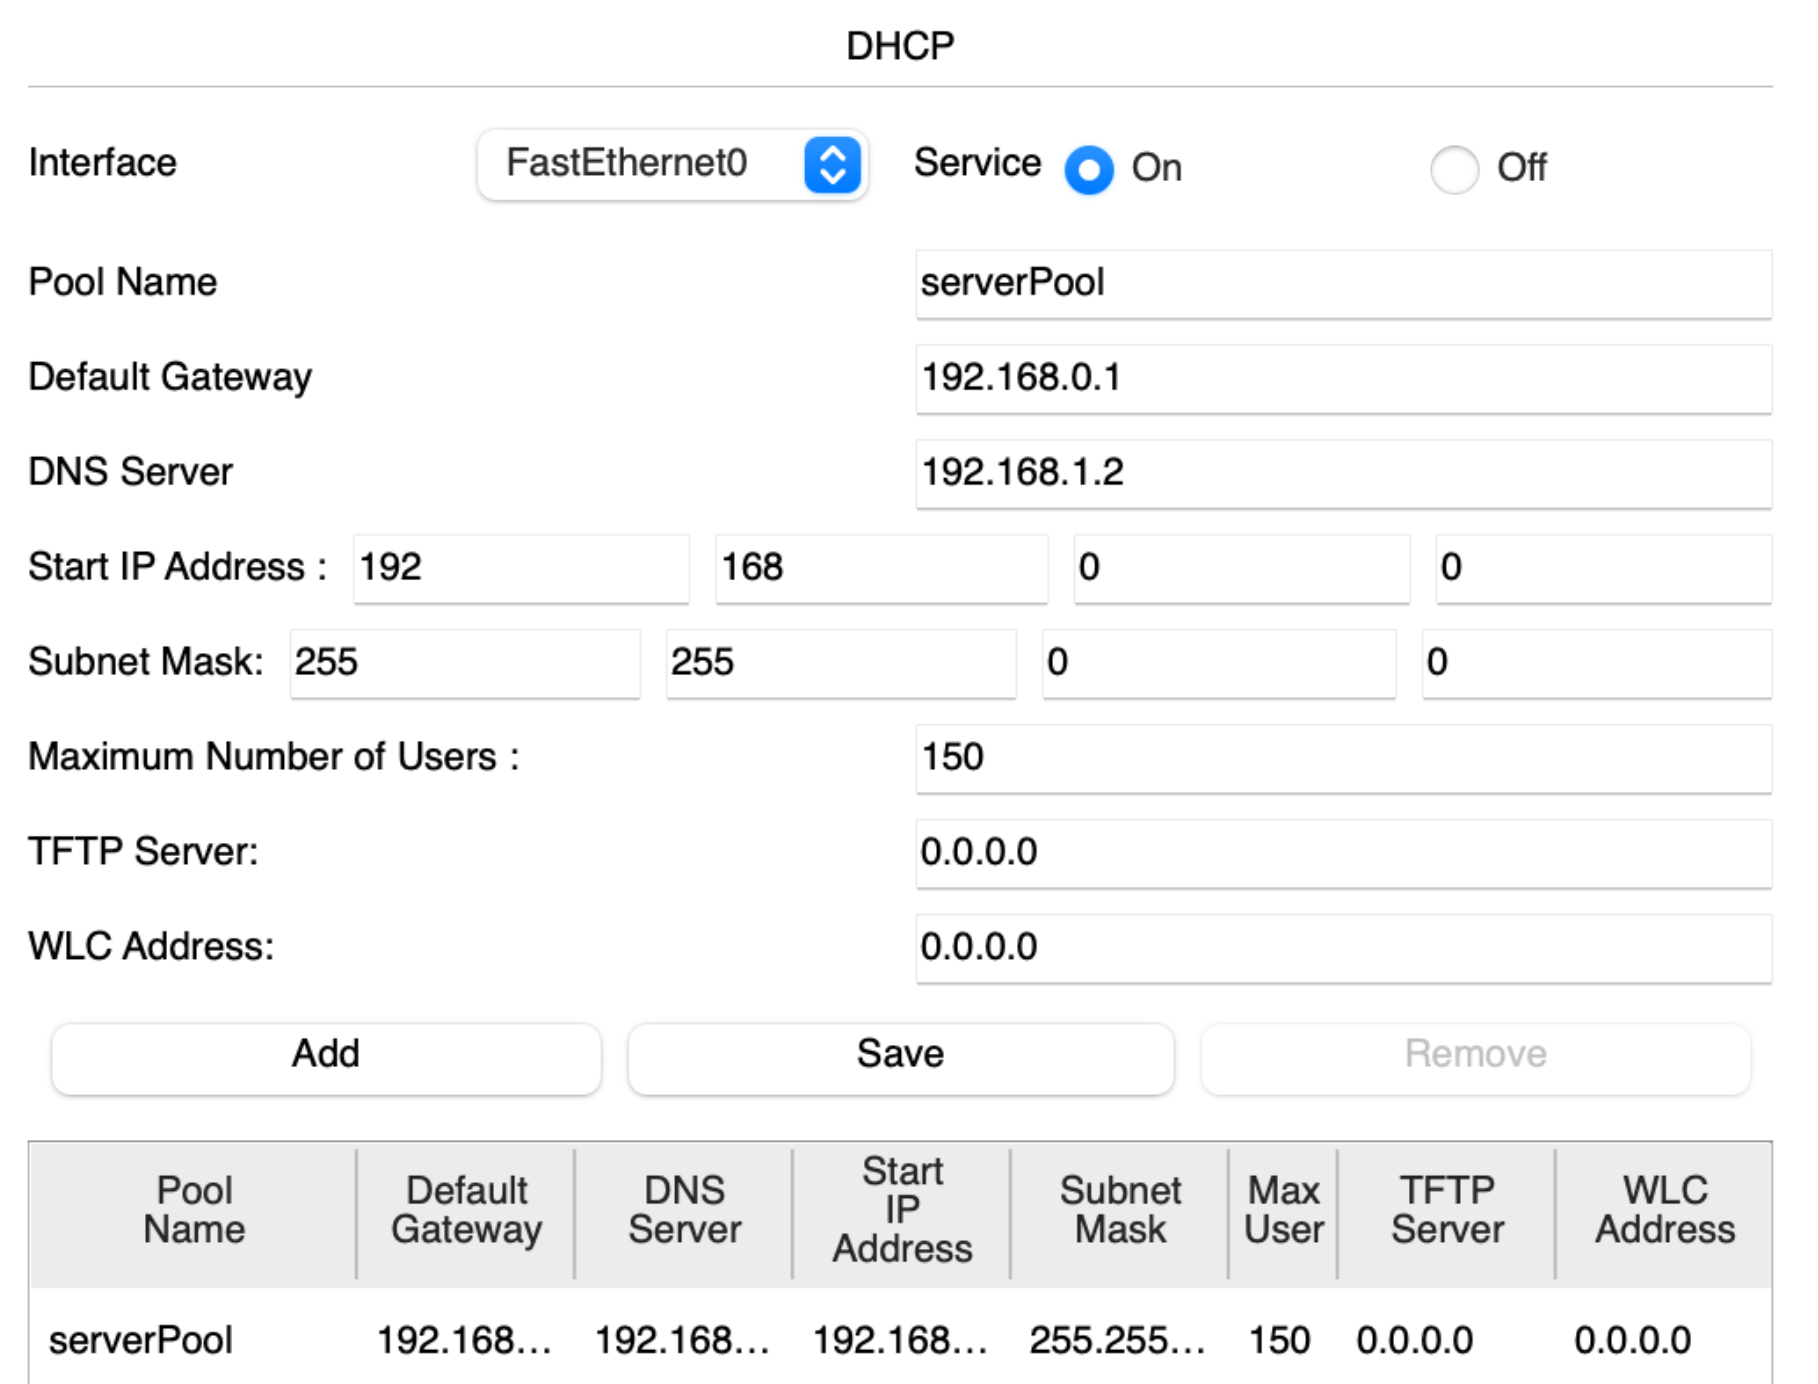
\includegraphics[width=0.65\textwidth]{lab-01-screenshots/41-5-DHCP-config.png}
    \caption{Configuración del servicio DHCP en el Server5.}
\end{figure}

\subsection{Asignación dinámica en clientes}

Cada usuario (PC1, PC2, PC3, PC4) fue configurado en modo DHCP. Al ejecutar seleccionar la opcion DHCP, se comprobó que los clientes recibieron direcciones dentro del rango definido, además del gateway y del servidor DNS.

\begin{figure}[H]
    \centering
    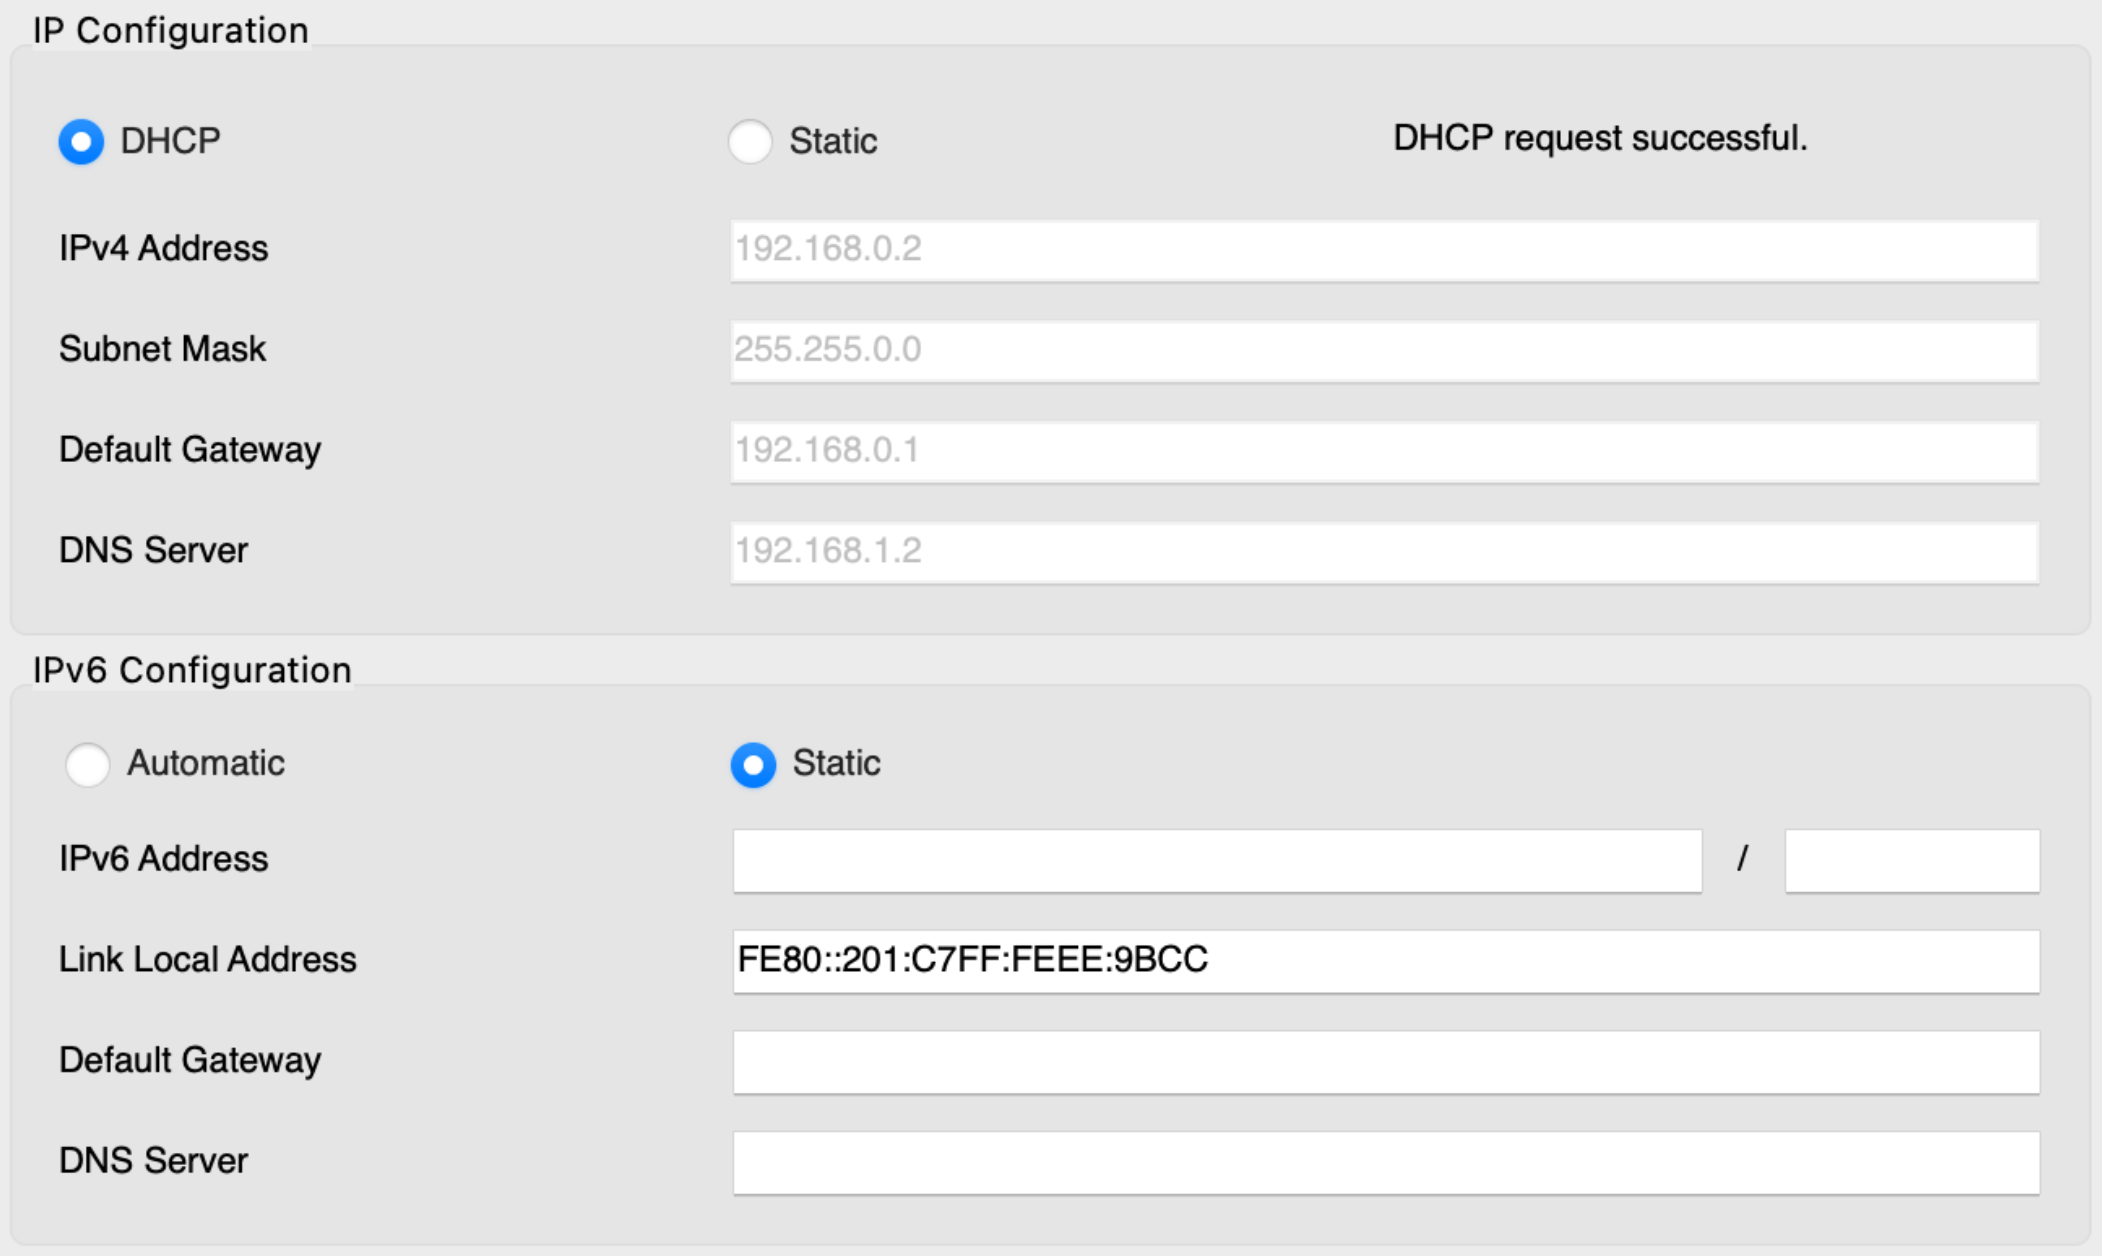
\includegraphics[width=0.65\textwidth]{lab-01-screenshots/41-6-user1-ip.png}
    \caption{Dirección IP obtenida dinámicamente por Usuario 1.}
\end{figure}

\bigskip
En conclusión, la red quedó con un direccionamiento mixto: los servidores con IP fija para garantizar disponibilidad, y los clientes con IP dinámica para mayor flexibilidad.

%==============================================================
%=====================   4.2   ================================
%==============================================================

\section{4.2 Configuración de servicio DNS}

El servicio DNS fue implementado en el Server1. Su propósito es \textbf{traducir nombres de dominio a direcciones IP}, de manera que los usuarios no tengan que recordar números, sino que puedan acceder a los servicios escribiendo su URL.

\subsection{Pasos realizados}

\begin{enumerate}
    \item Se deshabilitaron todos los servicios del servidor excepto el de \textbf{DNS}.
    \item En la pestaña de configuración de DNS, se agregaron registros de tipo \textbf{A Record}, asociando los nombres de dominio de los servicios con sus respectivas direcciones IP.
\end{enumerate}

\subsection{Registros configurados}

\begin{itemize}
    \item \texttt{dns.labredes.com} $\rightarrow$ 192.168.1.2
    \item \texttt{ftp.labredes.com} $\rightarrow$ 192.168.1.33
    \item \texttt{mail.labredes.com} $\rightarrow$ 192.168.1.34
    \item \texttt{web.labredes.com} $\rightarrow$ 192.168.1.35
\end{itemize}

\begin{figure}[H]
    \centering
    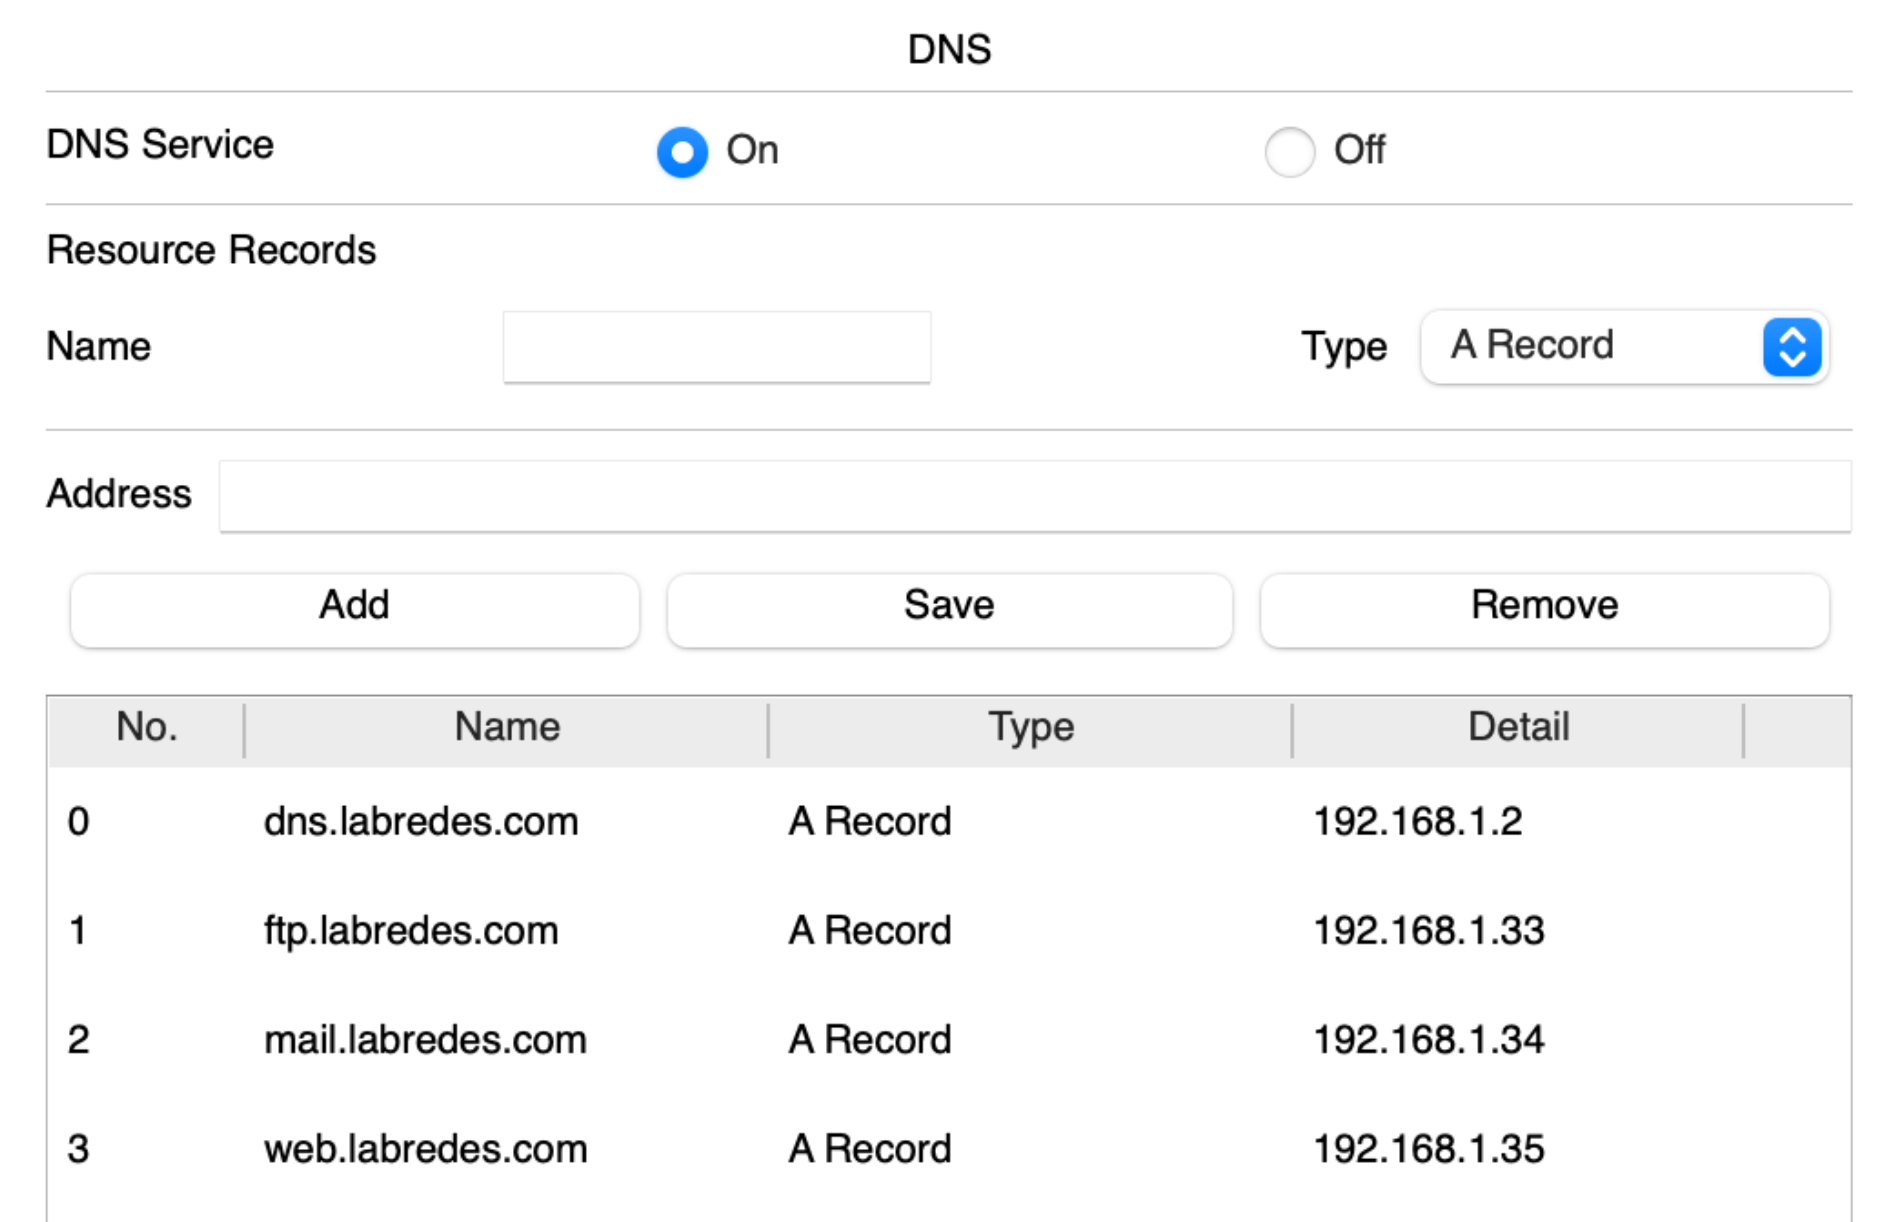
\includegraphics[width=0.65\textwidth]{lab-01-screenshots/42-1-DNS-config.png}
    \caption{Registros DNS configurados en el servidor.}
\end{figure}

\bigskip
Gracias a esta configuración, al realizar pruebas desde los clientes se logró acceder a los servicios tanto por dirección IP como por nombre de dominio. Esto demuestra el correcto funcionamiento del servidor DNS dentro de la red diseñada.

%==============================================================
%==================   RESTO SECCIONES   =======================
%==============================================================

\section{4.3 Pruebas de Conectividad (Comando ping) y Exploración del Protocolo DNS}
\section{4.4 Configuración y Exploración del servidor WEB}
\section{4.5 Configuración y exploración de los protocolos de correo electrónico SMTP y POP3}
\section{4.6 Configuración y exploración de protocolo FTP}

\end{document}
